
\chapter{Segmentation}

\section{Image Segmentation and Instance Segmentation}
\label{sec:image-segm-inst}

Image segmentation divides an image into several constituent regions.
The methods for this type of problem usually make use of the correlation between pixels in the image.
It does not need label information about image pixels during training, and it cannot guarantee that the segmented regions will have the semantics that we hope to obtain during prediction.

Instance segmentation is also called simultaneous detection and segmentation.
It studies how to recognize the pixel-level regions of each object instance in an image.
Different from semantic segmentation, instance segmentation needs to distinguish not only semantics, but also different object instances.


\section{Full Convolutional Network}
\label{sec:full-conv-netw}


Semantic segmentation focuses on how to divide an image into regions belonging to different semantic classes.
Different from object detection, semantic segmentation recognizes and understands what are in images in pixel level: its labeling and prediction of semantic regions are in pixel level.

The code is on \href{https://github.com/mingmingli916/segmentation}{Github}




\subsection{Transposed Convolution}
\label{sec:transp-conv}

Transposed convolution is shown in Figure \ref{fig:trans-conv}
\begin{figure}[!ht]
  \centering
  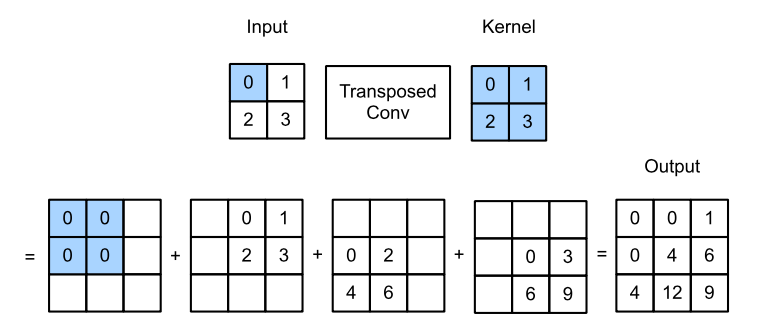
\includegraphics[width=0.8\textwidth]{transposed-conv}
  \caption{Transposed Convolution}
  \label{fig:trans-conv}
\end{figure}


\subsection{Fully Convolutional Networks}
\label{sec:fully-conv-netw}

A fully convolutional network (FCN) uses a convolutional neural network to transform image pixels to pixel classes.
Figure \ref{fig:fcn} shows the fully convolutional network.

\begin{figure}[!htbp]
  \centering
  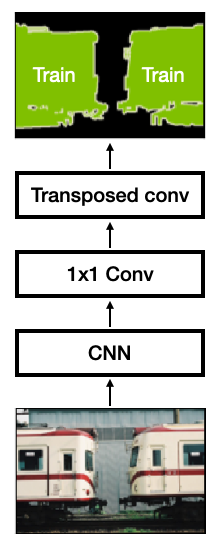
\includegraphics[width=0.3\textwidth]{fcn}
  \caption{FCN}
  \label{fig:fcn}
\end{figure}


%%% Local Variables:
%%% mode: latex
%%% TeX-master: "deep-learning"
%%% End:
